%!TEX root = ../../dissertation.tex
%%%%%%%%%%%%%%%%%%%%%%%%%%%%%%%%%%%%%%%%%%%%%%%%%%%%%%%%%%%%%%%%%%%%%%%%%%%%%%%
\chapter{Introduction}
\label{chap:intro}


\begin{itemize}
\item ARPANAT and evolutionary process to today's Internet scale
\item outside and inside developments brings new Internet usage (mp3+p2p, bandwidth+codecs -> video, digicams/camcorder); socioeconomic developments of a free speech network;New traffic patterns emerging due to external developments. Digital cameras, new codecs (esp MP3, mpeg4, WebM) -> p2p, Webcams 
\item mobile networks: more of a parallel development to the Internet, always centralized (from the old copper/telephony/circuit switched world)
\item MNs very different to the Internet structures we are used to
\item circuit switched roots, signaling, explicitly NOT a distributed system as compared to Internet, i.e. explicit signaling central controllers
\item Streaming and Multicasting, Multicasting in the Internet in general (only somewhat relevant for live/realtime non-interactive stuff)
\item content agnosticism: we do not know what applications the future will bring, so we do not make any assumptions
\item HTTP; ``The Web adopts relatively simple technologies with sufficient scalability efficiency and utility'' \cite{W3Arch}
\item Why HTTP streaming? Generalization of HTTP streaming (reliable transport, control shift to the client); Less control, more effective; Why global QoS control doesn't work
\item LTE, EPC, Core network tunneling concepts, bottlenecks in the access and the core, LTE network model
\item Improvements to congestion control for mobile streaming
\item Influence of L1/2/3 layer protocols and mechanisms (IPv4/6, tunneling, ethernet vs RLC/RRC/NAS, ...) ; what works better with it? compare, model and measure
\item QoE metrics, MOS, stalling time and buffering models, subjective and objective testing
\end{itemize}

%% new thesis stuff
Packet Switching, the process of chunking information into smaller bits, labeling it and transmitting it independently, was first described by Paul Baran in the 1960s\cite{baran1964distributed}. This changed communication a lot and provided one of the foundations for the emergence of the Internet. 


It was originally used to enable login to remote computers and soon thereafter remotely accessing files using FTP. But from it emerged countless other services and applications that are today used by hundreds of millions of people touching almost every aspect of daily life. 

The rise of the World Wide Web in the 1990s and even more in the last years made adoption of the Internet for the masses much easier. One needs just a single application to access and participate in most of the Internet's content in an easy accessible viewing format, i.e. the Web page defined with HTML.

External influences and developments also had a huge impact on the development of the Internet and the Web. E.g. it can be argued that the invention of MP3 audio compression lead to the development of peer-to-peer mechanisms and file sharing (Napster). The wide spread of digital cameras and camcorders was one of the pillars of success for social networks, including video streaming sites like YouTube.
A further requirements for these were the ever-increasing bandwidth capacities users had to access the Internet creating a two-way feedback loop. For every leap in bandwidth new services came up that filled it and fueling the users' demand for further capacity increases. 

Several factors contributed to the quick acceptance of the Internet. On the one hand, there are no assumptions made on the transported content. In contrast to the circuit switched telephone networks, which favor one mode of transportation and content (voice calls with specific procedures and/or codecs), in the Internet every packet is treated in the same way, leveling the playing field for every contender. On the other hand, one of the driving concepts of the Internet is the ``End-to-End Principle'' \cite{saltzer1984end2end, bhattacharjee1997active, blumenthal2001rethinking, isenberg1997rise, lemley2000end} which states:

``The function in question can completely and correctly be implemented only with the knowledge and help of the application standing at the endpoints of the communications system. Therefore, providing that questioned function as a feature of the communication system itself is not possible. (Sometimes an incomplete version of the function provided by the communication system may be useful as a performance enhancement)'' \cite{saltzer1984end2end} 

%%
network intelligence at the end nodes
--> end-to-end violations: ECN? only signaling, decision is e2e, same category as indirect TCP congestion control signaling (through loss) from the network
                           NAT, Firewalls?
Authors' 2000 followup \cite{reed2000endofe2e}
critical article \cite{moors2002critical}

Rethinking the design of the Internet: the end-to-end arguments vs. the brave new world \cite{blumenthal2001rethinking} : end-to-end enables the freedom to innovate and puts the choice of software and services completely to the user, no assumptions of the network have to be made
``[...] when are actions of an ISP responsible management, and when are they manipulative control of the nature and effective pricing of content and application?''
%%

This means, that functionality, i.e. services or applications, should only be implemented at the two endpoints of any packet flow. Making assumptions of the higher protocol layers and implementing functions in the network, essentially making it intelligent, will always only be valid for existing and narrow use cases and cannot support future developments. Despite critical arguments, e.g. in \cite{reed2000endofe2e, moors2002critical}, and mechanisms that superficially seem to violate it (NAT, ECN) this principle still drives progress in the Web.

The total volume if of Internet traffic has for many years been rising exponentially, as stated often fueled through external developments. The composition of today's traffic is manifold, but one large contributing factor is video. 
Video transport in the Internet is currently a topic of hot discussions. Older and well researched transport modes, e.g. RTP, are challenged by new ones, which integrate themselves better into the current web ecosystem. Yet, they use completely different approaches to streaming and the control thereof. This is also the first research interest of the doctoral thesis.
Streaming, or more generalized media transport is also not only relevant for the purpose of watching videos, there are many more fields of use which have slightly different requirements. With the popular cloud computing approach, which essentially means to run ones applications remotely on any number of hosts, it is necessary to transport the output of the applications, which often can be graphical, to the client. This is especially true for so-called Cloud Gaming services, which have hard temporal constraints on both directions of the transport path.

Mobile networks are still much closer to their circuit switching roots. Having evolved from GSM over UMTS to LTE, mobile networks have only very recently become fully packet switched. However, the data transport through its many core network elements is still using connection oriented techniques. The radio access' properties are also wildly different to traditional This poses unique challenges and opportunities for the design and performance of protocols. Therefore, we take a special interest in mobile network environments in our research of video streaming.

Concepts for future Internet structures are strongly disputed at the moment. A vast array of concepts is under discussion to either replace or enhance the protocol stack of the Internet's current setup. It will be interesting to measure the influence on media streaming and transport of these proposed changes or if there is any influence at all.


%%
Today, services based on the World Wide Web dominate the Internet's landscape. Especially noteworthy is the dominance of video streaming services in the traffic mixes of today and in future predictions (cf. Figures fig:netvine and fig:cisco). This development was supported through the availability of cheap and small digital camcorders and especially the now sufficient access bandwidth to support high quality video streams.
A similar development for cellular networks is now ongoing. Through the advent of affordable high performance smartphones and access technologies like UMTS and LTE many are now using their phones as the primary device for interacting with the Internet, including video streaming services such as YouTube, Netflix, or Hulu.

\begin{figure}[htbp]
    \centering
    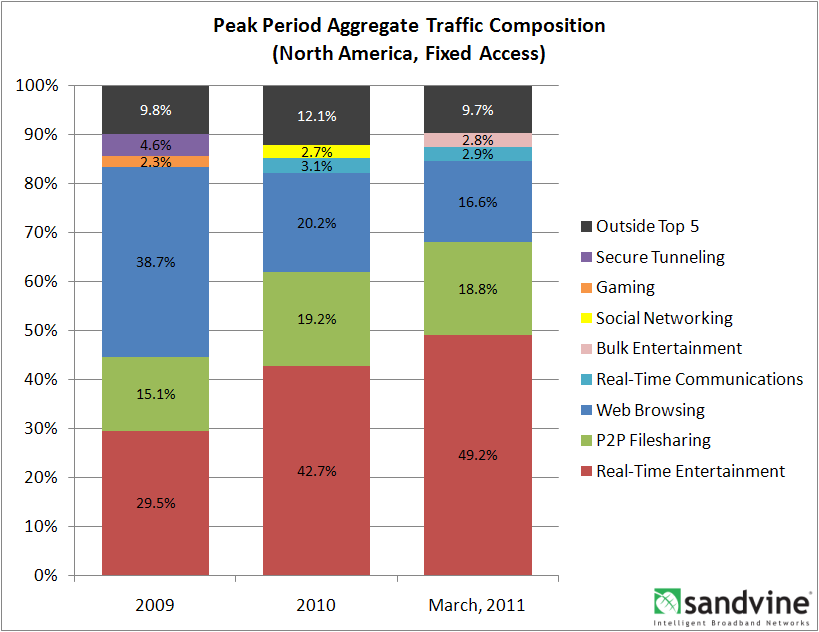
\includegraphics[width=0.8\textwidth]{images/netvine.png}
    \caption{Netvine, North American peak traffic (Source: \cite{sandvine_spring2011,sandvine_spring2013}).}
    \label{c1:fig:traffic_netvine}
\end{figure}

Figure~\ref{c1:fig:traffic_netvine} and Figure~\ref{c1:fig:traffic_cisco} ... TODO.

\begin{figure}[htbp]
    \centering
    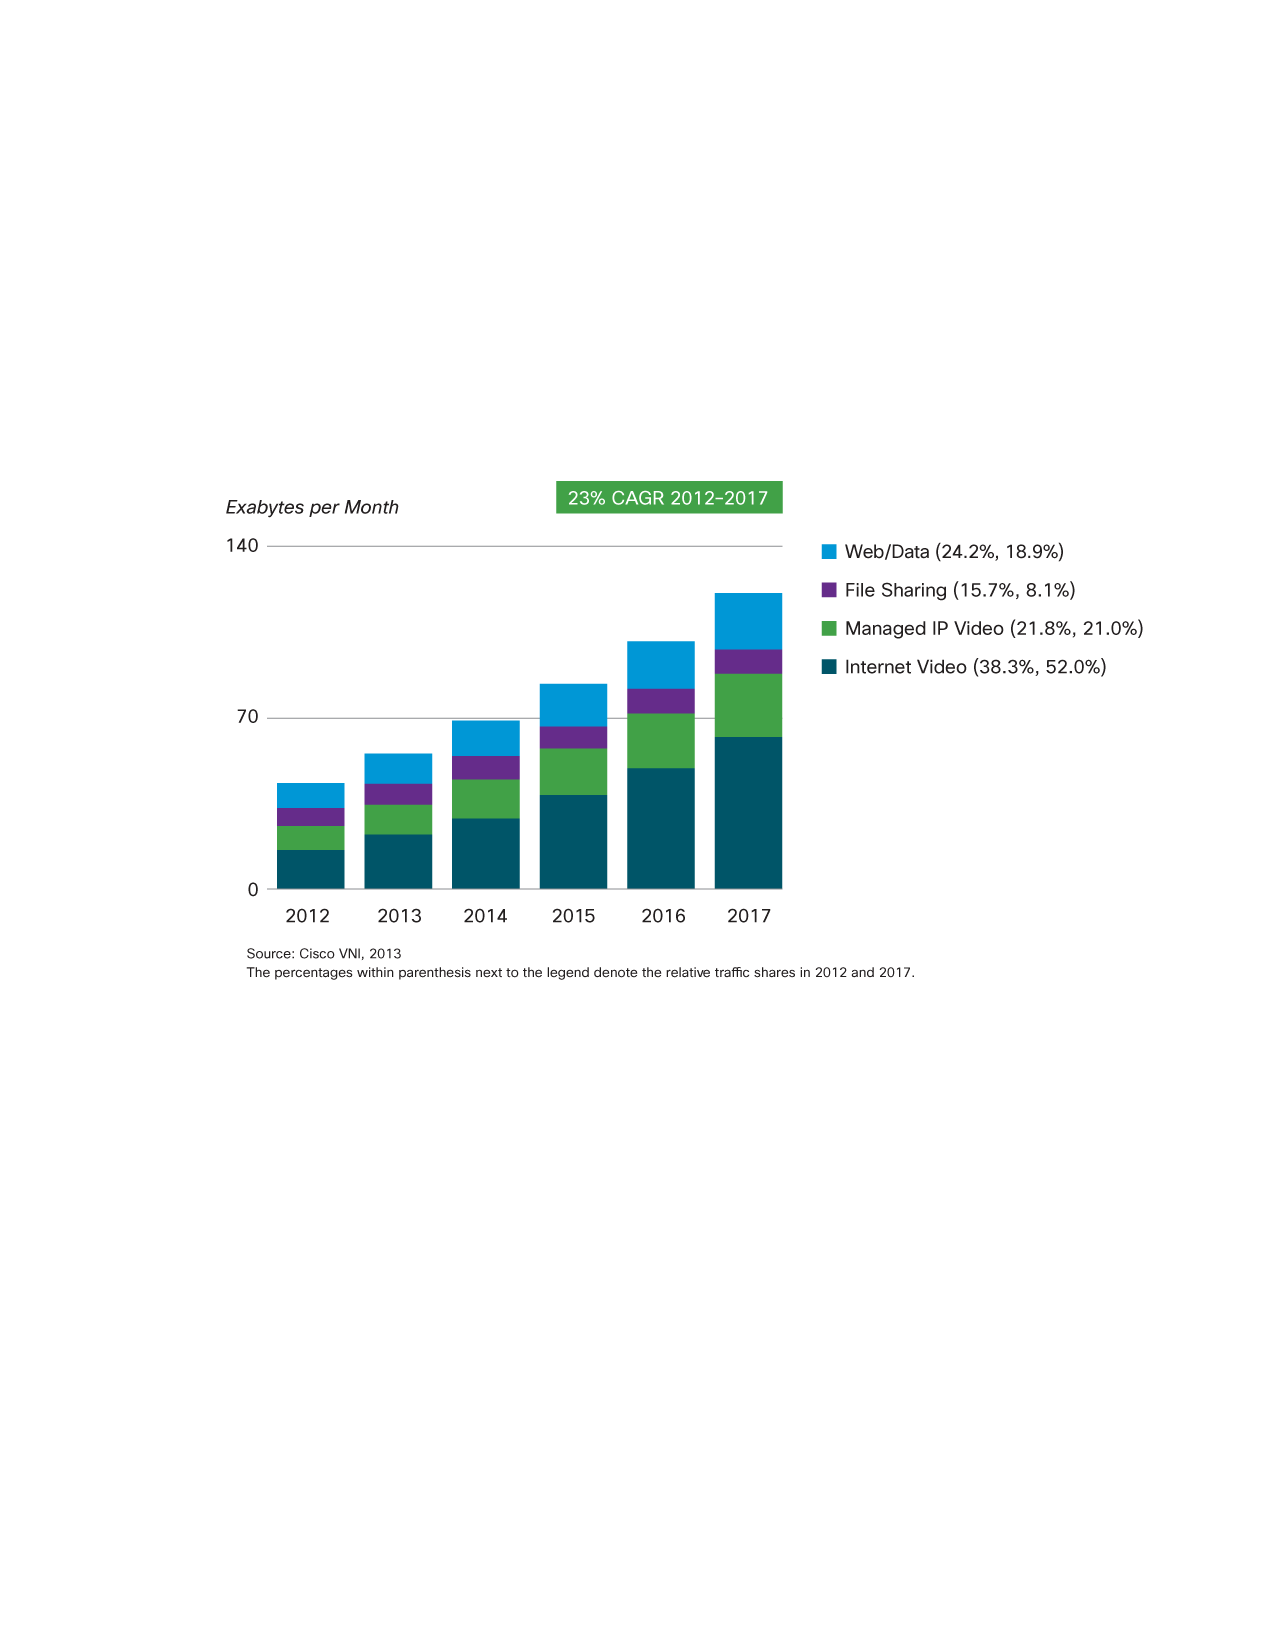
\includegraphics[width=\textwidth]{images/VNI_Hyperconnectivity_WP.pdf}
    \caption{Cisco, global consumer Internet traffic prediction (Source: \cite{cisco2013VNI}).}
	\label{c1:fig:traffic_cisco}
\end{figure}



This can put pressure on the overly complex cellular network structures. The radio transmissions have only access to a limited radio frequency spectrum that, moreover, has to be shared with any other phone user in the same cell. But there is also deemed to be significant pressure on the traffic management mechanisms of the mobile core networks backing up and aggregating the numerous radio cells of an operator. Little is known of the exact make-up of these networks as they are closely guarded secrets of the operator.

The popularity of these video services can to a degree be attributed to their full integration into the WWW. While previous offerings used completely different techniques which required the use of additional software, today one can enjoy videos just by directing ones browser to a website. Furthermore, other services related to video streaming are now also beginning to migrate to Web platforms. An example that is becoming increasingly popular at the moment are cloud gaming offerings which uses mechanisms very similar to real time video streaming but has stringent temporal constraints.


Most of today's services base itself on the Web and HTTP as ``transport protocol''. It is even proposed to use
a slightly modified version of HTTP as the basic end-to-end protocol for a future iteration of the Internet\cite{Popa:2010:HNW:1868447.1868453} as it already fulfills many of the demands proposed for the future of the Internet.


There are other applications closely related to video streaming and are showing similar transmission characteristics. Examples include remote desktop services or cloud gaming. Cloud gaming facilitates the same core principles as video streaming. However, it adds strong bidirectional real time requirements as user interaction needs to be immediately reflected in the streamed images. One of the concerns of the thesis could be an investigation of streaming models for cloud gaming in the context of mechanisms used . Initial work has already been done, e.g., in \cite{4795441,wang2009modeling,jarschel2011cloudevaluation,ct2010wolken}.



%%%%%%%%%%%%%%%%%%%%%%%%%%%%%%%%%%%%%%%%%%%%%%%%%%%%%%%%%%%%%%%%%%%%%%%%%%%%%%%%
\section{Motifs}




\subsection{Technical Solution Spaces}


\begin{figure}[htbp]
    \centering
    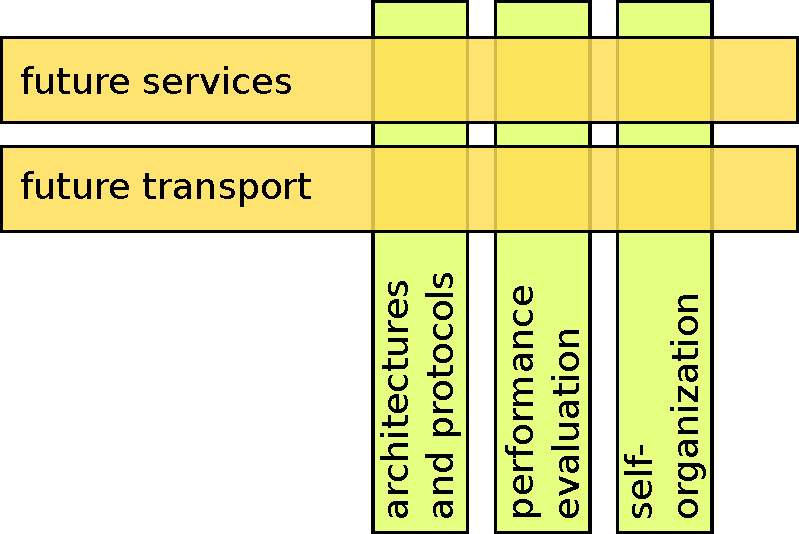
\includegraphics[width=.8\textwidth]{images/hv-topics-new.pdf}
    \caption{Technical solution spaces to the problem layers.}
    \label{c1:fig:hv-topics}
\end{figure}

As discussed, the core problems are layered into services and transport. Technologically, to solve the tasks of video streaming, one can approach these  threefold as displayed in Fig. \ref{c1:fig:hv-topics}.

The first is to dissect the involved protocols and architectures and break them down into their functional and methodical components. This will result in an improved understanding on the manner and process of their implementation. These components serve as building blocks for generalized models that abstracts the problem space from the actual implementation. The model will be defined by a set of parameters. To explore viable parameter ranges performance evaluation methods will be facilitated.


Secondly, using performance evaluation a system is methodically tested to the outcome of determining the influence of the system's parameters on a set of performance metrics. The parameters can be categorized into system intrinsic parameters, describing behavior only relevant and observable inside the system, and external parameters. In communication networks a good example for external parameters are the network Quality of Service parameters including latency, loss, jitter, and bandwidth capacity. Identifying fitting metrics for the measurement is a challenge. They can be either subjective or objective. The former are called Quality of Experience (QoE) metrics. They can only be measured by conducting empirical user studies and questionnaires and are mapped to a Mean Opinion Score (MOS). Extensive work has already been done to define baseline references for QoE metrics. Using these, one can directly translate objectively measurable outcomes into QoE metrics. However, these mappings may need to be adjusted to be able to handle stalling as the main source of quality loss. Examples for measuring subjective quality are available in \cite{gustafsson2008measuring, ketyo2010qoe}. 
Finally, one could employ methods of self-organization to try to reach improvements over conventional network setups.


\subsection{Apparatus for System Analyses and Comparison}

\begin{figure}[htbp]
    \centering
    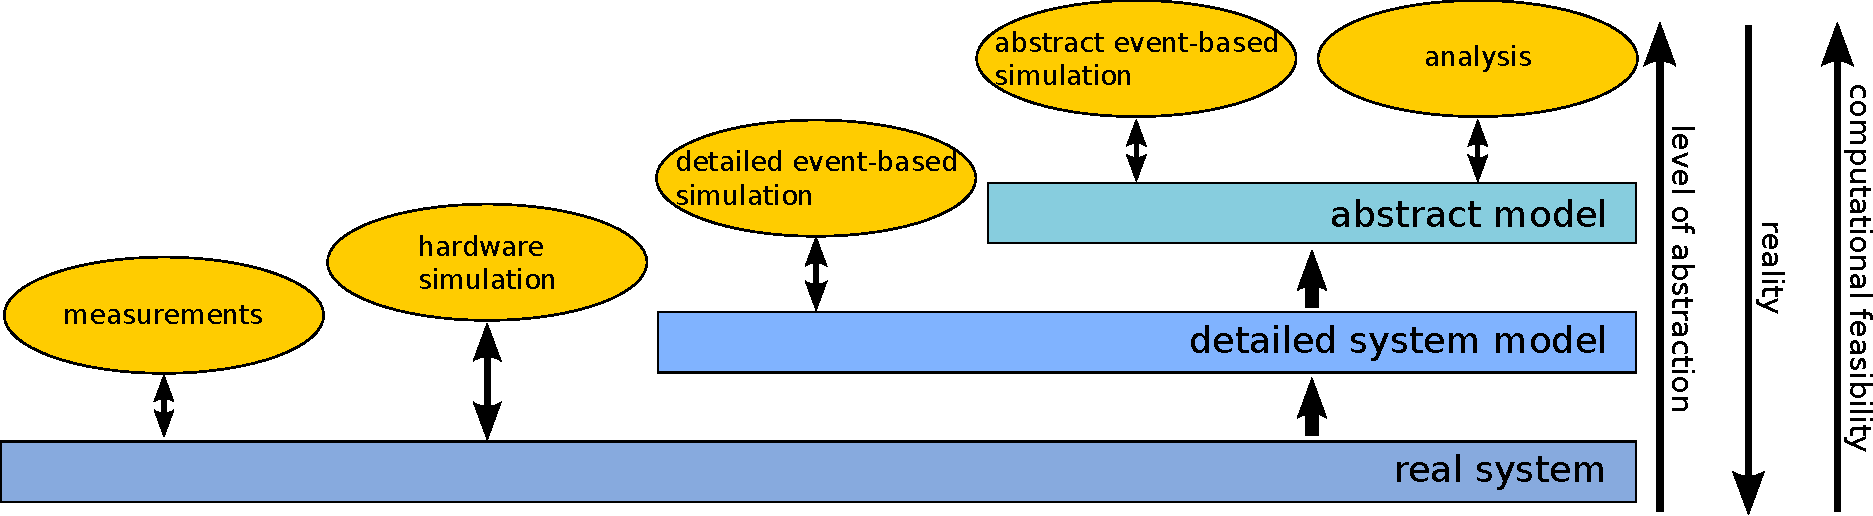
\includegraphics[width=1.0\textwidth]{images/apparatus-new.pdf}
    \caption{Methodical solution spaces and apparatus comparison.}
    \label{c1:fig:appcomp}
\end{figure}

Depicted in Figure \ref{c1:fig:appcomp} are levels of abstraction involved in system analysis and possible approaches to understand the system involved.

The upper limit for precision is achieved through actual measurements of the system itself. These give a point of reference and can be used to validate all other methods. However, this is not feasible to ascertain a larger view. The time frame or the physical size of the system is always limited.

Aside from measurements on implementations there are three further possible approaches which can widen the scope: emulation, simulation and mathematical analysis. 
Emulation tries to resemble implemented functionality as closely as possible while reducing the non-important parts to a minimum. Measurements using emulations can run in a normal network environment testbed and thus can only be done on a scale equivalent to implementations. The simulative approach implements all internal and external functionality, including the physical nodes and the network, in a discrete event simulation (DES). There may be subtle functional differences between a simulation and a real implementation. Therefore, validation is required. This approach benefits from the decoupling of the simulation from physical nodes as well as real time, allowing to measure large-scale networks in a short amount of time.
A mathematical analysis, for example using queuing theory and stochastic models, can then further broaden the understanding of the system.


The methods can all be used to define and explore solution spaces and are therefore important tools in understanding the problem. A fitting combination of these tools has to be found to advance the research. Our initial approach is to investigate existing streaming services, YouTube \cite{metzger2011delivery,mok2011measuring} and,e.g., video libraries of broadcast stations for simple HTTP streaming. A suitable candidate for measuring adaptive streaming still needs to be found as some candidate services apply regional restrictions. There are several reference applications available that implement different standardization approaches. These can be used to either directly measure the performance or to setup an emulation model based on their specifications.


\subsection{Further Approaches}
Further approaches which are under consideration, but will not be presented in detail here, are:

\begin{itemize}
\item Application of analytic and stochastic methods.
\item Formal definition of protocols or systems using Finite State Machines (FSM).
\item Creation of equivalent models.
\item Application of queuing theory, modeling the system through arrival processes, service time distributions and a number of servers and waiting places.
\item Data-mining of network trace data from mobile networks.
\end{itemize}



\subsection{Architecture and Protocols}

Mechanisms and protocols for the future of media streaming

\begin{itemize}
\item Compensation mechanisms for reliable transport
\item Model and quality estimations for improvements to adaptive streaming
\item End-to-end encryption and Authentication mechanisms (e.g.IPSec, DNSSEC, CurveCP) %(Daniel J. Bernstein)
\item Modifications to and issues with TCP
 \begin{itemize}
 \item TCP buffer bloat
 \item Initial window size (IW10, ...)
 \item WebSockets as streaming transport \cite{w3c2011websockets} \cite{heise2011websockets}
 \item WebRTC
 \item Relevance of multicasting or similar techniques for streaming transport (real-time live vs. stored)
  
 \item
 \end{itemize}
\item Service discovery and positioning (DNS modifications, CDNs, URIs, ``networking named content'')
\item Mobile networks
 \begin{itemize}
   \item Loss Hiding and conflict with congestion control mechanisms
   \item Shared media access, streaming with bandwidth/delay variations
   \item Mobility issues
     \begin{itemize}
       \item Mobility as a delay and loss source and its influence
       \item Investigation of mobility awareness and prediction techniques ("unassisted mobility")
     \end{itemize}
   \item future mobile networks
     \begin{itemize}
       \item Influence of control planes % Remove/Merge Control and User Plane
       \item Influence of (core) network elements (or a reduction thereof)
     \end{itemize}
 \end{itemize}

\end{itemize}




%%%%%%%%%%%%%%%%%%%%%%%%%%%%%%%%%%%%%%%%%%%%%%%%%%%%%%%%%%%%%%%%%%%%%%%%%%%%%%%%
\section{Goals and Aims}

The topic of the thesis will be the research of the inner workings of these new streaming services and mechanisms and especially its impact on the aforementioned cellular core network structures. This means conducting performance evaluations of the streaming mechanisms on itself and in the context of mobile networks as well as performing systematic assessments and classifications of the mechanisms. 

The result will be an understanding of the quantitative attributes related to these new forms of streaming. Furthermore, the thesis should provide tools and methods that help decide all participants of media streaming and mobile network operators which protocols and methods to choose and which are best suited for specific applications


%TODO:
    Performance analysis and comparison model of existing media streaming solutions
      But do not compare the protocols but the mechanisms and paradigms behind it
    Special focus on mobile environments and their pitfalls
    Improvements to protocols and new approaches

    Neue Videostreamingtechniken sind beliebt und bringen immer mehr Last in Mobilfunksysteme. Die Leistungsfähigkeit und die Qualität der Streaming-Dienste hängt insbesondere vom Verkehrsmanagement in Mobilfunksystem ab. Die Arbeit soll die Leistungsfähigkeit der neuen Streamingverfahren in heutigen und zukünftigen Mobilfunksystemen, die mit dem Internet verbunden sind, untersuchen. Die Schwierigkeit der Arbeit besteht in der Komplexität der Mobilfunksysteme und der neuen Streamingverfahren sowie in der Verknüpfungen der beiden Konzepte. Insbesondere die Auswirkung der Mobilfunkkernnetze auf die Leistungsfähigkeit der Mechanismen der Transportschicht sollen mit Hilfe von Methoden aus der Leistungsbewertung von Rechner- und Kommunikationsnetzen, untersucht werden.


On which kind of network information flow should streaming applications rely on in general and mobile networks specifically? What information is actually required for streaming?

What information flow should be provided by networks?

How can and should information be exchanged?

Can or should there be any dependence of the information flow on the application layer protocol?

How can the information flow be evaluated and modelled and the protocols and network architectures be compared? Is a generic evaluation model possible?

Design of new transport or streaming mechanisms
-> Formal Description Techniques

-> Analytical Tool, test viability


%%%%%%%%%%%%%%%%%%%%%%%%%%%%%%%%%%%%%%%%%%%%%%%%%%%%%%%%%%%%%%%%%%%%%%%%%%%%%%%%
\section{Structure}

This thesis is structured as follows.

The tackled protocols, systems, and mechanisms are described in Section X. Section Y details the methods that are and are planned to be used for the research. The final section gives a rough estimation on the thesis' schedule.